\chapter{Fundamentos teóricos}
\thispagestyle{empty}

? Distancia cámara sujeto

? Distorsión de perspectiva

? Reconocimiento facial

? Transferencia de aprendizaje

\section{Aprendizaje automático}
El aprendizaje automático (Machine Learning, ML) \cite{16,17} es una rama de la IA y de las ciencias de la computación centrada en el uso de datos y algoritmos para imitar la forma en la que los humanos aprenden, detectando patrones o regularidades para realizar predicciones.

Existen 3 tipos de aprendizaje dentro del ML \cite{18,19}:

El \textbf{aprendizaje supervisado} consiste en entrenar con datos de los que se saben sus etiquetas (una etiqueta nos indica qué es cada dato). Por ejemplo, los datos de entrada podrían ser imágenes de animales y sus etiquetas podrían ser "perro" o "gato". A partir de los datos y sus etiquetas, el agente aprende una función que dado un nuevo dato, predice su etiqueta. Es el tipo de aprendizaje más utilizado, los datos vienen ya 'preparados' para su uso. Es el tipo de aprendizaje que utilizaremos en este TFG.

En el \textbf{aprendizaje no supervisado} el agente aprende los patrones de los datos de entrada sin ninguna realimentación, es decir, los datos no están etiquetados. La herramienta más usada en el aprendizaje no supervisado es el agrupamiento, que consiste en detectar potenciales grupos en los datos de entrada. Este enfoque requiere un mayor número de datos.

En el \textbf{aprendizaje por refuerzo} el agente aprende mediante una serie de recompensas o castigos. El agente intentará realizar acciones que le proporcionen mejores recompensas en el futuro. Este tipo de aprendizaje es muy utilizado para enseñar a jugar a juegos.


\begin{comment}
\section{Visión por computador}
La visión por computador (VC) \cite{15} es un campo de la inteligencia artificial (IA) que permite a las computadoras y sistemas obtener información significativa a partir de imágenes digitales, vídeos y otras entradas visuales, y realizar acciones en base a esa información.

La visión por computador requiere una gran cantidad de datos. Realiza el análisis de los datos una y otra vez hasta que distingue diferencias o patrones y, en última instancia, reconoce imágenes. 

Se utilizan dos tecnologías esenciales para lograr esto: un tipo de aprendizaje automático llamado aprendizaje profundo (deep learning, DL) y las redes neuronales convolucionales (convolutional neuronal networks, CNNs).
\end{comment}


\section{Aprendizaje profundo}

\subsection{Redes neuronales}
Las redes neuronales (ANNs) \cite{24, 25} son redes computacionales que intentan, a groso modo, simular el proceso de decisión de las neuronas del sistema nervioso central de los animales o humanos. Las ANNs poseen unidades de procesamiento de información llamadas neuronas, que están conectadas entre sí mediante capas. La red se compone de (ver Figura \ref{fig3}):
\begin{itemize}
	\item Una capa de entrada, que tendrá tantos inputs como características o variables tenga el problema
	\item Una o varias capas ocultas, compuestas por neuronas. El número de capas ocultas define la profundidad de la red neuronal.
	\item Una capa de salida, que representa el valor o valores predichos
\end{itemize} 

\begin{figure}[h]
	\centering
	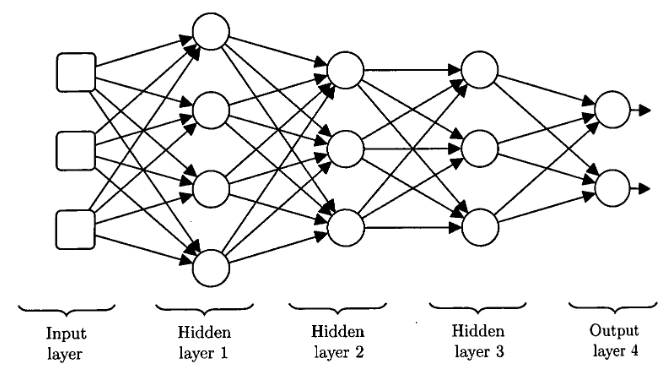
\includegraphics[scale=0.5]{imagenes/cap2/neural-network.png}
	\caption{Esquema de una red neuronal \cite{26}.}
	\label{fig3}
\end{figure}

Las neuronas son la unidad fundamental de cómputo, tienen varios valores de entrada y un valor de salida que se conecta con las neuronas de la siguiente capa. Los elementos básicos del modelo neuronal son (ver Figura \ref{fig4}:

\begin{itemize}
	\item Un conjunto de conexiones con las señales de entrada. Cada conexión tiene su propio peso/fuerza.
	\item Una función de suma de las señales de entrada, ponderadas cada una con su peso. Estas operaciones constituyen una combinación lineal.
	\item Una función de activación, para limitar la amplitud de la salida de la neurona. Normalmente, el rango de salida está en el intervalo [0,1], o alternativamente en [-1,1]. Existen muchos tipos de funciones de activación pero, se suelen utilizar tres: la función signo, la función logística y la función arco-tangente.
\end{itemize} 

\begin{figure}[h]
	\centering
	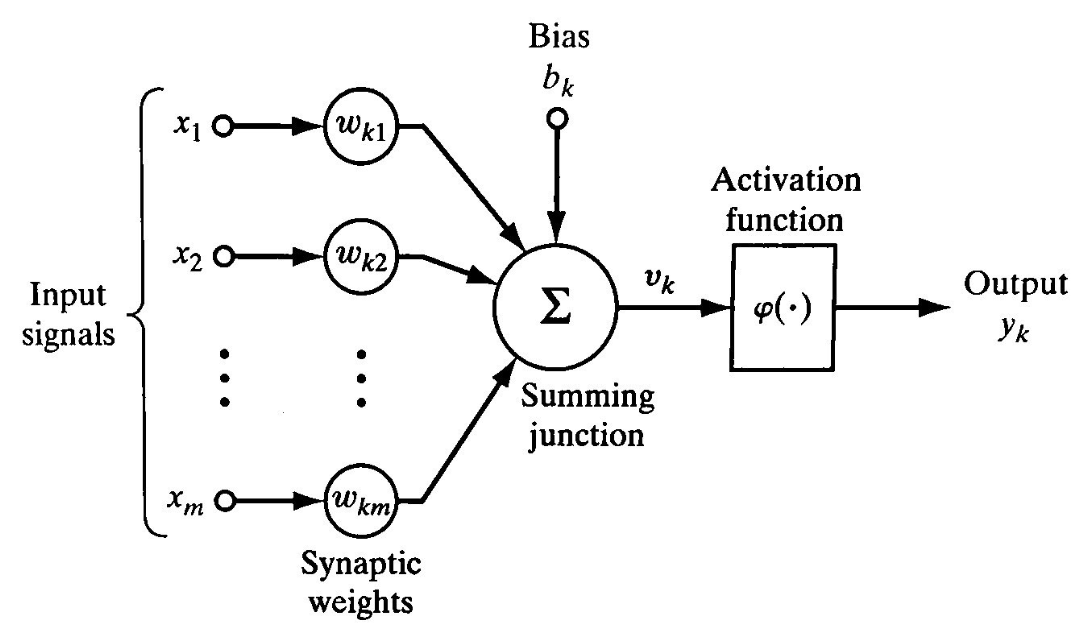
\includegraphics[scale=0.25]{imagenes/cap2/neuron-model.png}
	\caption{Modelo neuronal para una neurona k \cite{25}.}
	\label{fig4}
\end{figure}

En términos matemáticos, podemos describir la salida de una neurona como:

\begin{equation}
	y = \phi(\sum_{j=1}^{m} w_j x_j + b)
\end{equation}

siendo $\phi$ la función de activación, $m$ el número de señales de entrada, $w_j$ el peso de cada entrada $x_j$, y $b$ el sesgo.

El algoritmo de aprendizaje de la red neuronal consiste en ir modificando los pesos y el sesgo, iterativamente, hasta alcanzar el resultado deseado. Este proceso iterativo se conoce como entrenamiento, y permite, a través de las modificaciones de los pesos, reconocer y extraer las características más relevantes de los datos.

El objetivo del entrenamiento es minimizar el error de predicción de la salida de la red neuronal, para ello, se define una función de pérdida. Existen numerosas funciones de pérdida, algunas de las más conocidas son: el error cuadrático medio (MSE), el error absoluto medio (MAE) o la entropía cruzada. La información de la función de pérdida se transmite desde la salida a la capa inicial, con el fin de adecuadamente los pesos para generar una mejor estimación de la predicción.

Es importante encontrar un equilibrio entre generalización y sobreentrenamiento. Generalizar demasiado implica que el modelo es muy simple y no es capaz de captar patrones en los datos. Mientras que, el sobreentrenamiento, provoca que al recibir nuevos datos no utilizados para entrenar, se estime un mal resultado debido a la poca capacidad de generalización ante nuevos datos.


\subsection{Redes neuronales convolucionales}


\subsubsection*{Capa de pooling}